\subsection{Retriving the physical location of the interventions}
\label{sec:dist_mat}
Some information that the challenge providers have access to, such as the physical location of each intervention, is not public. This will be later on used to compute the environmental impact and the concurrency of close interventions. In order to determine a plausible physical location of the interventions, a two step approach is proposed: first the relative positioning between interventions must be determined, then these positions should be aligned with the map of France. Making some assumptions will allow us to extract this meaningful information from the available data while maintaining the integrity of the original problem structure.\\

We will start with the assumption that there is a component of the risk that comes from the location of an intervention. This is intuitive since interventions in densely populated areas or near critical infrastructure likely carry higher risks than those in remote locations. However, it is important to notice that location is not the only factor, the risk also depends on other variables like the type of maintenance work. \\ 

\begin{assumption}
  Two interventions \(i\) and \(j\) are close if their overall mean risks (averaged accross all possible start times and scenarios)
  \[
  \overline{r}_t^{(i)} = \frac{1}{\left|\mathcal{T}_i\right|}\sum_{\mathcal{T}_i}\mu_t^{(i,\tau)}, 
  \qquad \text{where }\mu_t^{(i,\tau)} \coleq \frac{1}{|S|}\sum_{s\in S} \mathrm{risk}_{s,t}^{(i,\tau)}, \quad
  \mathcal{T}_i\coleq \{\tau\in \N:\,1\leq \tau \leq T-d_{i,\tau}\}
  \]
  vary in the same direction, i.e.,
  \[
  \operatorname{sgn}\Big(\overline{r}_{t+1}^{(i)}-\overline{r}_t^{(i)}\Big)=\operatorname{sgn}\Big(\overline{r}_{t+1}^{(j)}-\overline{r}_t^{(j)}\Big),\quad t\in\{1,\dots , \mathcal{T}-1\}
  \]
  This affirms that the risk variation of an intervention over time is strongly correlated with its location.
\end{assumption}


In practice, this condition will rarely hold for all time periods $t$. However, we can use it to define a similarity measure between interventions by counting how often their risk variations align. Specifically, for each pair of interventions $(i,j)$, we compute a similarity score by adding 1 when their risk variations match in sign and subtracting 1 when they differ. Then it is normalized to the interval $[-1,1]$. This yields a symmetric similarity matrix that captures the degree of correlation between intervention risks over time.

\begin{remark}
    By definition, an intervention has a correlation of 1 with itself.
\end{remark}

Notice that not all correlation values provide information about the closeness between interventions. Only positively correlated interventions can be considered ``close" to some extent. However, we cannot determine how far apart negatively correlated interventions should be. Therefore, these negative correlations will be set to \texttt{NaN} and treated as missing values.\\

There is not enough information to assign a specific distance value between 2 close points, but following assumption 1: the higher the correlation between two interventions, the stronger the indication that they are close to each other. Therefore, the algorithm proposed to recover a map from a distance matrix is: non-metric weighted Multi-Dimensional Scaling (MDS):

\begin{itemize}
    \item \textbf{MDS:} Given a distance matrix (or dissimilarity matrix), it minimizes a stress function (\ref{eq:stress}) to find an embedding in a specified number of dimensions (in our case, 2 dimensions).
    \item \textbf{Non-metric:} Instead of using the magnitude of the distances, it only considers the ordinal information induced by those values. Higher correlations indicate closer distances, but the size of the difference between correlations is not necessarily proportional to the actual distances between interventions.
    \item \textbf{Weighted:} Each distance's contribution to the stress function is weighted by its correlation value, reflecting higher confidence in our assumption when correlations are stronger.
\end{itemize}

\begin{remark}
    The dissimilarity/distance matrix is obtained through a linear transformation of the previously defined similarity matrix:
    \begin{align*}
        \text{NaN} &\rightarrow \text{NaN} \\
        \text{cor}_{ij} &\rightarrow \text{dist}_{ij} = 1-\text{cor}_{ij}, \quad \text{where } \text{cor}_{ij} \in [0,1]
    \end{align*}
\end{remark}


\subsubsection*{Non-metric Weighted MDS with SMACOF \cite{smacof}:}
\paragraph{Problem Formulation.} Let us assume we have $n$ objects, and an $n\times n$ matrix of observed dissimilarities 
\[
\Delta = \bigl[\delta_{ij}\bigr],
\]
where $\delta_{ij} \ge 0$ and each pair of objects $(i,j)$ is assigned a weight $w_{ij}\ge 0$. The goal of \emph{non-metric} weighted MDS is to find an embedding of these objects as points $\mathbf{x}_1,\dots,\mathbf{x}_n$ in $\mathbb{R}^p$ (collectively denoted by $X \in \mathbb{R}^{n\times p}$), such that the pairwise distances $d_{ij}(X) = \|\mathbf{x}_i - \mathbf{x}_j\|$ (usually Euclidean) respect the \emph{rank ordering} of $\delta_{ij}$.

Formally, non-metric MDS replaces $\delta_{ij}$ with a \emph{monotonic transformation} $f(\cdot)$, yielding
\[
\hat{\delta}_{ij} = f(\delta_{ij}),
\]
subject to the isotonic constraint:
\[
\delta_{ij} < \delta_{kl} 
\quad \Longrightarrow \quad 
f(\delta_{ij}) \;\le\; f(\delta_{kl}).
\]
In case of a tie $(\delta_{ij} = \delta_{kl} )$, disparities are allowed as long as they maintain the correct ordering with respect to non-tied values.

We then define the \emph{weighted STRESS} function:
\begin{equation}
\mathrm{STRESS}(X,\hat{\Delta}) 
\;=\;
\frac{\sum_{i<j} w_{ij}\,\bigl(\hat{\delta}_{ij} \;-\; d_{ij}(X)\bigr)^2}{\sum_{i<j} w_{ij}\,d_{ij}(X)^2},
\label{eq:stress}
\end{equation}
where $\hat{\Delta}$ denotes the matrix $\bigl[\hat{\delta}_{ij}\bigr]$.  
The goal is to minimize this STRESS with respect to both $X$ and the (monotonic) mapping $f$. Missing values are simply not taken into account in the sum (which is equivalent to setting their weight to 0).

\paragraph{Solution via SMACOF}\label{sec:smacof-solution}
\emph{Scaling by MAjorizing a COmplicated Function} is an iterative algorithm that provides a stable, monotone-convergent framework for MDS. Unlike Kruskal's classic method, which uses gradient-based updates to move the configuration $X$, SMACOF replaces the gradient step with a \emph{majorization step} that guarantees non-increasing STRESS accross iterations. This is typically more numerically stable and better at handling large amounts of missing data.

The algorithm alternates between two main steps:

\begin{enumerate}
  \item \textbf{Initialization}
    \begin{enumerate}[(a)]
      \item Collect all non-missing dissimilarities $\{\delta_{ij}\}$ and set the corresponding weights $w_{ij}$ (with $w_{ij}=0$ for missing values).
      \item Choose an initial configuration $X^{(0)} \in \mathbb{R}^{n \times p}$ (e.g., via random placement or classical MDS).
    \end{enumerate}

  \item \textbf{Iterative Steps}
    \begin{enumerate}[(a)]
      \item \textbf{Optimal Scaling (Isotonic Regression):} \\
      Given the current configuration $X^{(t)}$, compute the Euclidean distances
      \[
        d_{ij}\bigl(X^{(t)}\bigr)=\|x_i^{(t)} - x_j^{(t)}\|,
      \]
      and determine the disparities by solving
      \[
        \min_{f\,:\, \text{non-decreasing}} \sum_{i<j} w_{ij}\,\Bigl(f(\delta_{ij}) - d_{ij}\bigl(X^{(t)}\bigr)\Bigr)^2.
      \]
      In practice, weighted isotonic regression (e.g., via the Up-and-Down-Blocks Algorithm\footnote{Up-and-Down-Blocks is a specific implementation strategy for PAVA (Pool-Adjacent-Violators Algorithm) that can be optimized for efficiency and linear time complexity. There are other possible implementations of PAVA that could be used.\cite{PAVA}}, see algorithm \ref{algo:Up-and-Down-Blocks}) is applied to obtain $\hat{\delta}_{ij}=f(\delta_{ij})$, ensuring that the transformed dissimilarities preserve the original rank order.
      
      \item \textbf{Majorization Update (Guttman Transform):} \\
      With the disparities $\hat{\Delta}=\{\hat{\delta}_{ij}\}$ fixed, 
      SMACOF constructs a quadratic majorizing function $Q\bigl(X, X^{(t)}\bigr)$ satisfying
      \[
        \mathrm{STRESS}(X,\hat{\Delta}) \le Q\bigl(X, X^{(t)}\bigr), \quad \text{with equality when } X = X^{(t)}.
      \]
      Minimizing $Q\bigl(X, X^{(t)}\bigr)$ leads to a closed-form update via the Guttman transform:
      \[
        X^{(t+1)} = V^{+}B\bigl(X^{(t)}\bigr)X^{(t)},
      \]
      \hspace{1em}where the constant matrix \(V\) is defined by
          \[
            V = \frac{1}{2}\sum_{i=1}^n \sum_{j=1}^n w_{ij}\,A_{ij}, \qquad \text{where }A_{ij} = (e_i - e_j)(e_i - e_j)^T,
          \]
          \hspace{1em}with \(e_i\) denoting the \(i\)th standard basis vector. Note that \(A_{ij} = A_{ji}\), and \(A_{ii} = 0\). The factor \(\frac{1}{2}\) accounts for double counting of symmetric terms. \(V\) is positive semidefinite and singular. Its Moore-Penrose inverse is denoted by \(V^{+}\).\\

        \hspace{1em}And the matrix \(B\bigl(X^{(t)}\bigr)\) is defined element-wise by
          \[
            B\bigl(X^{(t)}\bigr) = \frac{1}{2} \sum_i \sum_j w_{ij} \, \hat{\delta}_{ij} \, s_{ij}\bigl(X^{(t)}\bigr) \, A_{ij}, \quad \text{where } s_{ij}\bigl(X^{(t)}\bigr) = \begin{cases} \dfrac{1}{d_{ij}\bigl(X^{(t)}\bigr)} & \text{if } d_{ij}\bigl(X^{(t)}\bigr) \neq 0, \\ 0 & \text{otherwise} \end{cases}
          \]
          \hspace{1em}where \(d_{ij}\bigl(X^{(t)}\bigr)\) is the Euclidean distance between points \(i\) and \(j\) in the current configuration.

      By construction, the update satisfies
      \[
        \mathrm{STRESS}\bigl(X^{(t+1)},\hat{\Delta}\bigr) \le \mathrm{STRESS}\bigl(X^{(t)},\hat{\Delta}\bigr),
      \]
      ensuring a monotone decrease in stress.
    \end{enumerate}

  \item \textbf{Convergence Check}
    \begin{enumerate}[(a)]
      \item After updating $X^{(t+1)}$, recompute the stress. If the reduction in stress is below a predetermined tolerance (or no further improvement is observed), terminate the algorithm; otherwise, set $t\leftarrow t+1$ and return to the Optimal Scaling step.
    \end{enumerate}
\end{enumerate}


For details about the global linear convergence to a stationary point conditions of SMACOF see \cite{smacof}.

\begin{algorithm}[!ht]
    \caption{Up-and-Down-Blocks Algorithm for Isotonic Regression \cite{modernMDS}}
    \label{algo:Up-and-Down-Blocks}
    \KwIn{A distance matrix $D=\{d_{ij}(X)\}$ from the current configuration $X$, and corresponding rank-ordered proximities $\{\delta_{ij}\}$ (with possible ties).}
    \KwOut{Disparities $\{\hat{d}_{ij}\}$ that are monotonic (non-decreasing) with respect to $\delta_{ij}$.}
    
    \tcp{Step 1: Initialization}
    \For{each pair $(i,j)$}{
        Set $\hat{d}_{ij} \gets d_{ij}(X)$\;
    }
    
    \tcp{Step 2: Iterative Pooling to Enforce Monotonicity}
    \While{there exists an index $k$ such that $\hat{d}_k > \hat{d}_{k+1}$}{
        \tcp{(a) Identify the first (leftmost) violation and initialize block $B$.}
        Let $k$ be the smallest index with $\hat{d}_k > \hat{d}_{k+1}$\;
        Set $B \gets \{k, k+1\}$\;
        Compute the block average:
        \[
        \bar{d} \gets \frac{\hat{d}_k + \hat{d}_{k+1}}{2}\,.
        \]
        and for each $i \in B$, set $\hat{d}_i \gets \bar{d}$\;
        
        \tcp{(b) Extend the block to the left.}
        \While{there exists an index $j = \min(B)-1$ such that $\hat{d}_j > \bar{d}$}{
            Update $B \gets B \cup \{j\}$\;
            Recompute 
            \[
            \bar{d} \gets \frac{1}{|B|}\sum_{i \in B} \hat{d}_i\,,
            \]
            and for each $i \in B$, set $\hat{d}_i \gets \bar{d}$\;
        }
        
        \tcp{(c) Extend the block to the right.}
        \While{there exists an index $l = \max(B)+1$ such that $\bar{d} > \hat{d}_l$}{
            Update $B \gets B \cup \{l\}$\;
            Recompute 
            \[
            \bar{d} \gets \frac{1}{|B|}\sum_{i \in B} \hat{d}_i\,,
            \]
            and for each $i \in B$, set $\hat{d}_i \gets \bar{d}$\;
        }
    }
    
    \tcp{Step 3: Handling Ties}
    For tied proximities (i.e., when $\delta_{ij} = \delta_{kl}$), the algorithm enforces overall monotonicity; that is, it does not explicitly force $\hat{d}_{ij} = \hat{d}_{kl}$. (If needed, a reordering step can ensure that disparities for tied proximities remain in non-decreasing order.)
    
    \tcp{Step 4: Normalization (for SMACOF/MDS)}
    Scale the final disparities so that
    \[
    \sum_{i<j} \hat{d}_{ij}^2 = \frac{n(n-1)}{2}\,.
    \]
    
    \Return $\{\hat{d}_{ij}\}$\;
\end{algorithm}

\begin{figure}[!ht]
    \centering
    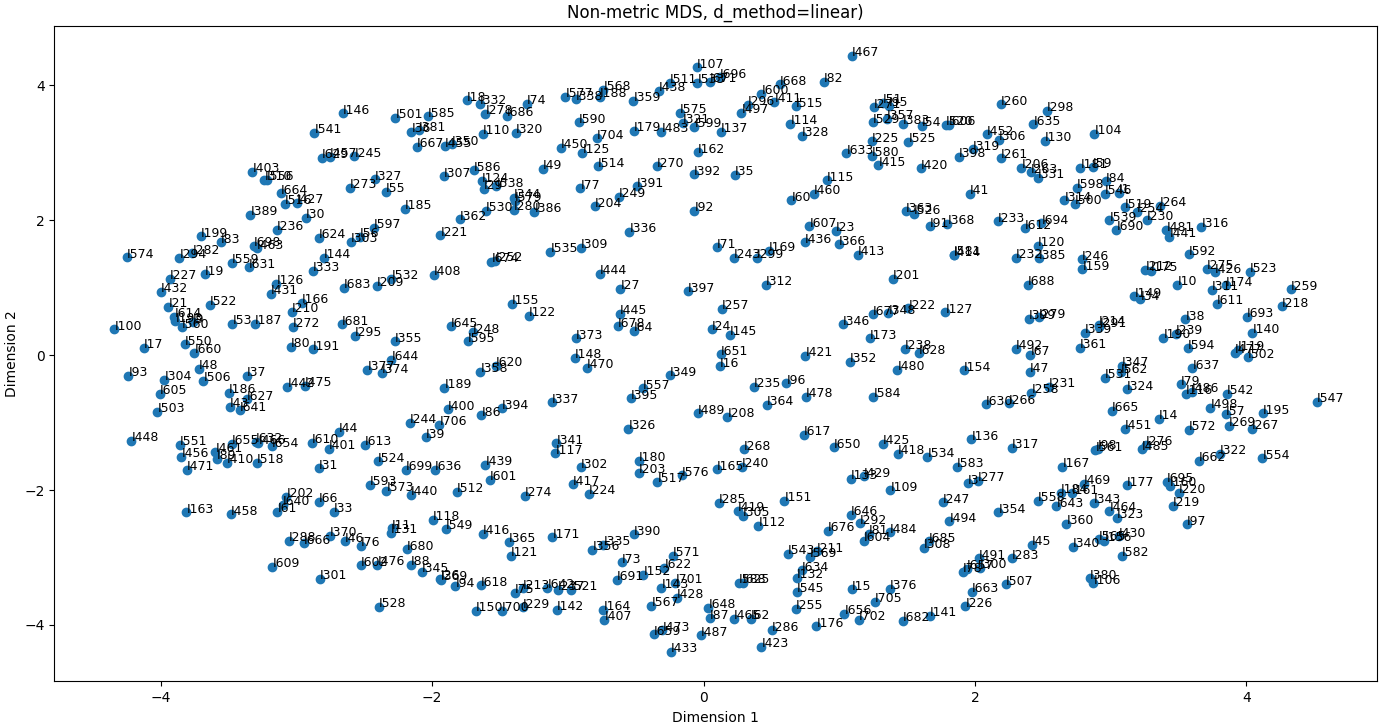
\includegraphics[width=\textwidth]{ch3/figures/points.png}
    \caption{Visualization of the resulting MDS map showing the relative positions of the interventions from \texttt{X12} in a two-dimensional space based on their dissimilarities derived from assumption 1.}
    \label{fig:mds_map}
\end{figure}

Once the cloud of points (i.e. the distance matrix) is obtained via SMACOF, the next step involves placing those points on the map of France, enabling the computation of distances to national parks. Since no intervention property can be directly linked to a specific geographical position, the approach consists of isotropically stretching (uniformly in both axes) and translating the cloud of points onto the French map, as illustrated in Figure \ref{fig:map_france}. While this reconstruction is not intended to substitute actual geographical data, it provides a solid and justified foundation for subsequent spatial analysis within the constraints of the problem.

\begin{figure}[!ht]
    \centering
    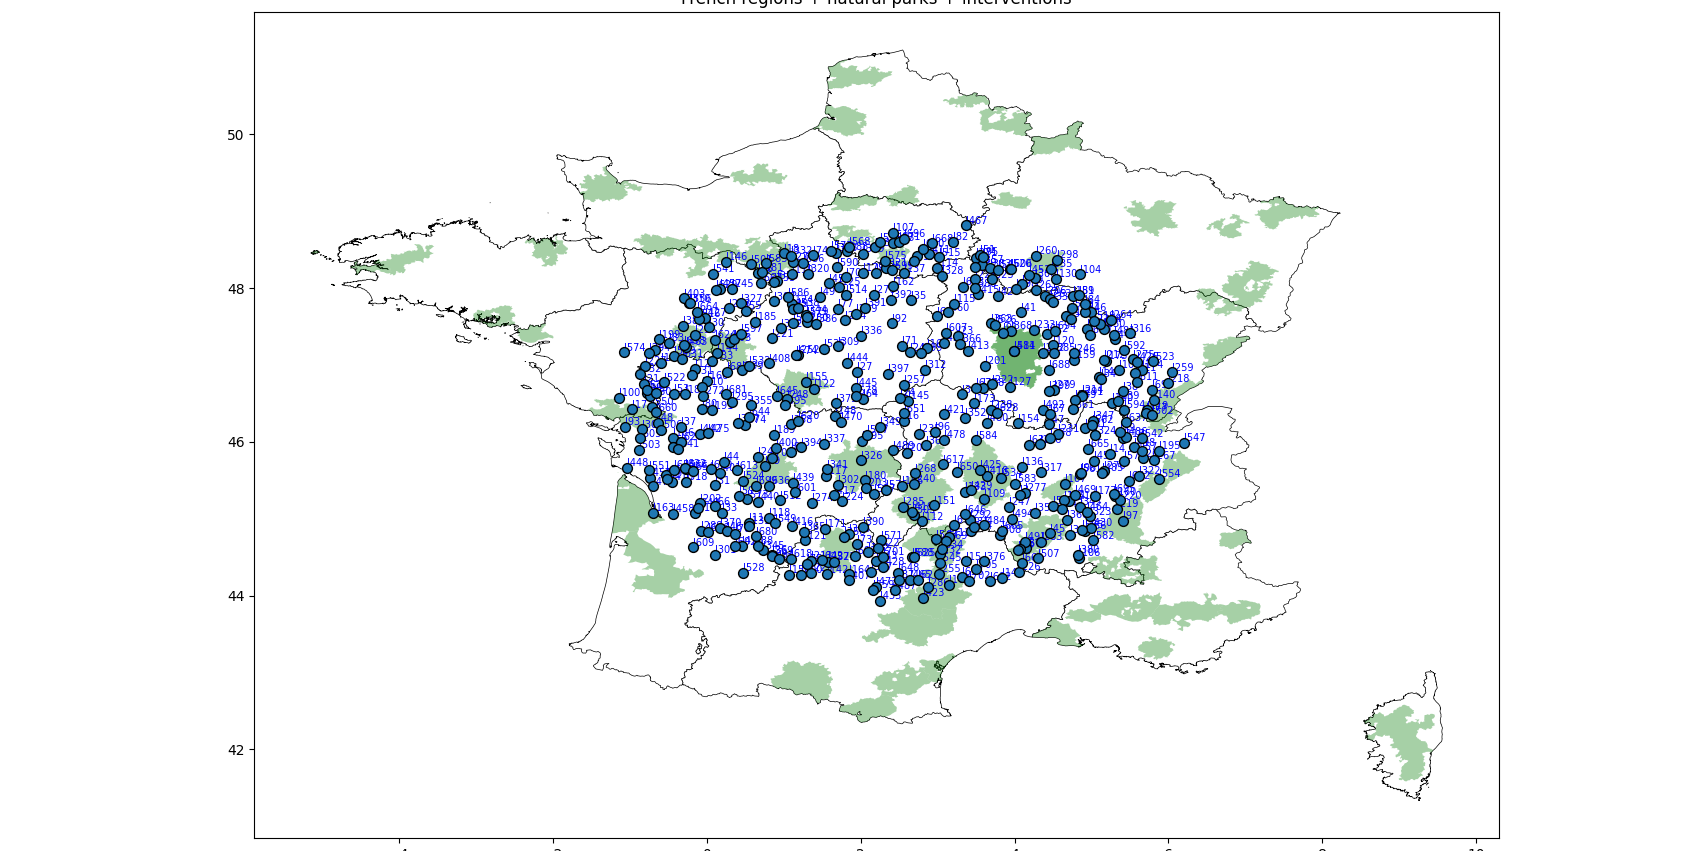
\includegraphics[width=\textwidth]{ch3/figures/Map of France.png}
    \caption{Visualization of the intervention locations after stretching and translating the MDS point cloud to fit the French territory. Green areas represent the regional natural parks.}
    \label{fig:map_france}
\end{figure}


